%$Id: lattice.tex,v 1.1 1992/05/10 19:39:06 rz Exp rz $

\chapter{Lattice Techniques}
\label{Lattice:Chap}

Thus far we have considered diophantine approximation problems where
we are trying to find good approximations to a single irrational
number $\alpha$.  This can be expressed as determining integers $p$
and $q$ that minimize $|q \alpha - p|$.  Continued fraction techniques
can be used to efficiently determine integers $p$ and $q$ satisfying
\begin{equation} \label{1D:Approx:Eq}
\left| q \alpha - p\right| \le \frac{1}{q}.
\end{equation}
This is a rewritten form of \propref{CF:RatApprox:Prop}.

When more than one irrational number is involved, there are two
natural ways to generalize \eqnref{1D:Approx:Eq}.  Let $\alpha_1,
\ldots, \alpha_n$ be irrational numbers.  We can find integers $p_{1},
\ldots, p_{n}, q$ that minimize
\begin{equation}
\left| q \alpha_{i} - p_{i} \right|
\label{Simul:Approx:Eq}
\end{equation}
or those that minimize
\begin{equation}
\left|p_0 + p_{1} \alpha_{1} + p_{2} \alpha_{2} + \cdots + p_{n} \alpha_{n} \right|.
\label{Linear:Form:Eq}
\end{equation}
The problem of finding the $p_{i}, q$ that minimize
\eqnref{Simul:Approx:Eq} is called a \keyi{simultaneous approximation 
problem}, while finding the $p_{i}$ that minimize
\eqnref{Linear:Form:Eq} is called the\index{linear form problem} {\em
linear form problem\/}.  {\Dirichlet} resolved both of these problems in
1842 \cite{Dirichlet1842-es} by proving the following two propositions.

\begin{proposition}[{\Dirichlet}] 
\label{Dirichlet:Multiple:Prop}
Given irrational numbers $\alpha_{1}, \ldots, \alpha_{n}$ there exist
an infinite number of sets $\{p_{1}, \ldots, p_{n}, q\}$ such that
\[
\left| q \alpha_{i} - p_{i}\right| \le q^{-1/n}
\]
\end{proposition}

When $n = 1$ this gives the same result as \longpropref{CF:RatApprox:Prop}. 

\begin{proposition}[{\Dirichlet}]
\label{Dirichlet:Mutual:Prop}
Given real numbers $\alpha_{1}, \ldots, \alpha_{n}$ and an
$\epsilon$ in the open interval $(0, 1)$ there exist $p_{0}, p_1,
\ldots, p_{n}$ with $\left|p_{i}\right| \le \epsilon^{-1/n}$ such that
\[
\left| p_0 + p_{1} \alpha_{1} + p_{2} \alpha_{2} + \cdots + p_{n} \alpha_{n} \right|
\le \epsilon
\]
\end{proposition}

\begin{figure}
\begin{center}\tabcolsep=2pc
 \begin{tabular}{cc}
  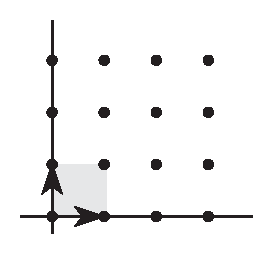
\includegraphics{lbasisa} 
   &
  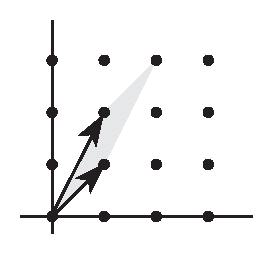
\includegraphics{lbasisb} \\
  (a) & (b)
 \end{tabular}
\end{center}
\caption{Two different bases for ${\protect\Z} \times {\protect\Z}$
     \label{Lattice:Basis:Fig}}
\end{figure}

A new geometric method of proving these results was given by {\Minkowski}
by his development of the \key{geometry of numbers}.  In this chapter
we follow {\Minkowski}'s lead and use these geometric techniques.  A
significant advantage of the geometric approach is the recent
development of (relatively) efficient algorithms for solving
multidimensional approximation problems like those mentioned above.
In addition to solving problems in diophantine approximation, these
algorithms can also be used to find relations between numbers and to
factor polynomials. 

\section{Lattice Fundamentals}
\label{Lattice:Fund:Sec}

The elements of $\mathbb{R}^{n}$ are $n$-tuples that for an additive group by 
component-wise addition. Multiplication by an element $a \in \mathbb{R}$ 
maps $\vec v = \langle v_1, v_2, \ldots, v_n \rangle \in \R^n$ to 
$a \vec v = \langle av_1, av_2, \lodts, a v_n \rangle$.

A \keyi{lattice} is a discrete subset of $\mathbb{R}^{n}$ that 
can be generated by $n$ linearly independent vectors: 
\begin{equation*}
{\cal L} = \{\, \lambda_{1} \vec b_{1} + \cdots + \lambda_{n} \vec b_{n} \mid
\lambda_{i} \in \Z \,\}.
\end{equation*}
We call $\{\vec b_{1}, \ldots, \vec b_{n}\}$ a {\em
basis}\index{lattice!  basis of} of the lattice ${\cal L}$.  As illustrated
in \figref{Lattice:Basis:Fig}, a lattice can have more than one basis.
In this case, the lattice is ${\cal L} = \Z \times \Z$.  In
\figref{Lattice:Basis:Fig}(a) we have shown the natural basis $\vec b_{1} =
(1, 0)$ and $\vec b_{2} = (0, 1)$, while \figref{Lattice:Basis:Fig}(b)
shows the alternative basis $\vec b_{1}' = (1, 2)$ and $\vec b_{2}' = (1, 1)$.
 
Each of these two figures includes a shaded parallelepiped defined by
the two basis vectors.  Each shaded region is called the
\keyi{fundamental domain} of the corresponding basis.  Repeated copies
of the fundamental domain \key{tessellate} $\mathbb{R}^{n}$.  As we shall see,
the volume of fundamental domain of a lattice is independent of the
basis used to define it.

The geometric properties of a lattice are induced by the definition
used for distance.  For all applications with which we are concerned,
the distance between two points is invariant under rigid translations
of the two points.  Thus the distance between the two points $\vec{x}$
and $\vec{y}$ is the length of the vector between them---that is, the
length of $\vec{x}-\vec{y}$.  When given suitable properties, a function
that maps vectors in $\Re^n$ into their length is called a \textbf{norm}.
We will only consider distance measures that are derived from norms.

\begin{definition}
A {\bf norm}\index{norm! of a lattice} on $\mathbb{R}^{n}$ is a map 
$d: \mathbb{R}^{n} \rightarrow \mathbb{R}$ such that 
\begin{enumerate}
\item $d(x) \ge 0$ for all $x \in \mathbb{R}^{n}$,
\item $d(x) = 0$ if and only if $x = 0$,
\item $d(\alpha x) = |\alpha| d(x)$, for $\alpha \in \mathbb{R}$,
\item $d(x+y) \le d(x) + d(y)$.
\end{enumerate}
\end{definition}

Each of these conditions has a natural geometric interpretation.  The
first two conditions say that the length of every vector other than
$(0, \ldots, 0)$ is positive.  The third says that if we scale the
entire space by a factor of $\alpha$ then the length of the vector
increases by a factor of $|\alpha|$.  The fourth condition is the
triangle inequality.

A frequently used collection of norms are the {\em
$p$-norms},\index{p-norm of a lattice@$p$-norm of a lattice} which are
denoted by $\|\;\|_{p}$.  If $x = (x_{1}, \ldots, x_{n})$ is a point
in $\mathbb{R}^{n}$, then $\|x\|_{p}$ is defined to be
\[
\|x\|_{p} = \sqrt[p]{|x_{1}|^{p} + |x_{2}|^{p} + \cdots + |x_{n}|^{p}}.
\]
Useful special cases of the $p$ norm are the $1$-norm of $x$,
$\|x\|_{1}$; the \keyi{Euclidean norm}, $\|x\| = \|x\|_{2}$; and the
maximum norm $\|x\|_{\infty}$.  The $1$-norm of $x$ is defined by
\[
\|x\|_{1} = |x_{1}| + |x_{2}| + \cdots + |x_{n}|,
\]
which is the ``Manhattan'' length of $x$.\index{Manhattan length} The
Euclidean distance function\index{Euclidean distance} is just the $2$-norm:
\[
\|x\|_{2} = \sqrt{|x_{1}|^{2} + |x_{2}|^{2} + \cdots + |x_{n}|^{2}}.
\]
The \keyi{maximum norm} is the limit of $\|x\|_{p}$ as $p$ goes to
infinity:
\[
\|x\|_{\infty} = \max (|x_{1}|, \ldots, |x_{n}|).
\]
All of the $p$-norms generate the same topology on $\mathbb{R}^{n}$.
\addsymbol{$\|\vec{v}\|_p$}{$p$ norm of a vector}
\addsymbol{$\|\vec{v}\|$}{$2$ norm of a vector, Euclidean distance}
\addsymbol{$|\vec{v}|$}{$\infty$ norm of a vector, sum of absolute
values of its components}

The fact that the $p$-norms are norms follows from the \keyi{Minkowski
inequality} \cite[pages 115--117]{Minkowski2018-iz}:

\begin{proposition}[{\Minkowski}]
If $x_1, \ldots, x_n$ and $y_1, \ldots, y_n$ are non-nega\-tive real
numbers, then for all $p \ge 1$
\[
\left(|x_1 + y_1|^p + \cdots + |x_n + y_n|^p\right)^{1/p} \le 
\left(x_1^p + \cdots + x_n^p\right)^{1/p} + 
\left(y_1^p + \cdots + y_n^p\right)^{1/p}.
\]
\end{proposition}

\noindent
A proof of this proposition can be found in \cite{Hardy1952-ad}.\Marginpar{Include the proof here.}

Determining whether a set of points is a lattice can be quite
difficult, if the set is not specified in terms of set of basis
vectors.  In this situation the following proposition is quite useful.
For a proof see {\Cassels} \cite[page 78]{Cassels2012-kd}.

\begin{proposition} \label{Lattice:Condition:Prop}
A necessary and sufficient condition that a set of points ${\cal L} \subset
\mathbb{R}^n$ be a lattice is that the set satisfy:
\begin{itemize}
\item ${\cal L}$ is closed under component-wise addition,
\item ${\cal L}$ contains $n$ linearly independent points,
\item There exists a constant $\eta> 0$ such that if $(x_1, \ldots,
x_n) \in {\cal L}$ and
\[
\sqrt{x_1^2 + \cdots + x_n^2} < \eta,
\]
then $x_1 = x_2 = \cdots = x_n = 0$.
\end{itemize}
\end{proposition}

The first two conditions ensure that there is a basis for the points
of ${\cal L}$.  The third condition states that there is a neighborhood of
the origin that contains only one point.  This ensures that all the
points of ${\cal L}$ are separated and thus the basis is a $\Z$ lattice.

\paragraph{Fundamental Domains}

\begin{figure}
\begin {center}
 \begin {tabular}{cc}
   \begin{picture}(150, 62)
     \put(0,0){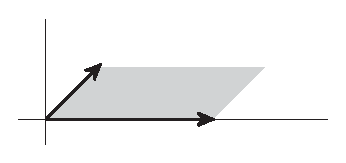
\includegraphics{FundDoma}}
     \put(85,0){$\vec{a}$}
     \put(30,42){$\vec{b}$}
   \end{picture}
  & 
   \begin{picture}(150, 62)
     \put(0,0){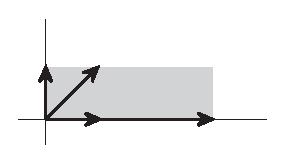
\includegraphics{FundDomb}}
     \put(100,0){$\vec{a}$}
     \put(40,42){$\vec{b}$}
     \put(40,0){$\vec{b}_{\parallel}$}
     \put(3,42){$\vec{b}_{\perp}$}
   \end{picture} \\
   (a) & (b) 
 \end{tabular}
\end{center}
\caption{Computing the Area of a
Parallelogram\label{Lat:Parallel:Fig}}
\end{figure}

The volume of the fundamental domain is an important property of a
lattice.  As we shall show, it does not depend on the basis, but is an
invariant of the lattice.  If the basis vectors are orthogonal then
the volume of fundamental domain is just the product of the lengths of
the vectors.  Recall that two vectors $\vec{a}$ and $\vec{b}$ are
orthogonal if and only if their {\em dot product}\index{dot product!of two
vectors} vanishes
\[
\vec{a} \cdot \vec{b} = a_1 b_1 + \cdots + a_n b_n = 0.
\]
To compute the volume of a general parallelepiped we modify
the basis vectors in such a way that the volume is left unchanged, but
the new vectors are orthogonal.  This is illustrated in
\figref{Lat:Parallel:Fig}. 
\addsymbol{$\vec{a}\cdot\vec{b}$}{Dot product of $\vec{a}$ and
$\vec{b}$, $a_1 b_1 + \cdots + a_n b_n$}

The area of the parallelogram bounded by the vectors $\vec{a}$ and
$\vec{b}$ is the same as that of the rectangle in
\figref{Lat:Parallel:Fig}(b).  In \figref{Lat:Parallel:Fig}(b), we
have decomposed $\vec{b}$ into the sum of two orthogonal vectors
$\vec{b}_{\perp}$ and $\vec{b}_{\parallel}$.  $\vec{b}_{\parallel}$ is
the portion of $\vec{b}$ that is parallel to $\vec{a}$ and does not
contribute to the area of the parallelogram.  Thus, the area delimited
by $\vec{b}_{\perp}$ and $\vec{a}$ is the same as that
delimited by $\vec{a}$ and $\vec{b}$.  The magnitude of
$\vec{b}_{\parallel}$ is $\vec{b} \cdot \vec{a}$, so 
\[
\vec{b}_{\perp} = \vec{b} - \frac{\vec{b} \cdot \vec{a}}{\|\vec{a}\|} \,
\frac{\vec{a}}{\|\vec{a}\|} = 
\vec{b} - \frac{\vec{b} \cdot \vec{a}}{\vec{a} \cdot \vec{a}}\,
\vec{a}\;,
\]
where the second factor is the unit vector parallel to $\vec{a}$.
So, if we denote by $\vec{b}^{\ast} = \vec{b}_{\perp}$ and
$\vec{a}^{\ast} = \vec{a}$ the orthogonalization of $\vec{a}$ and
$\vec{b}$ we have
\[
\left(\begin{array}{c} \vec{a} \\ \vec{b} \end{array}\right)
= 
\left(\begin{array}{cc} 1 & 0 \\ 
\frac{\vec{b} \cdot \vec{a}}{\vec{a} \cdot \vec{a}} & 1 \end{array}\right)
\cdot
\left(\begin{array}{c} \vec{a}^{\ast} \\ \vec{b}^\ast \end{array}
\right)
\]
More generally, we can orthogonalize the vectors $\vec{a}_1, \ldots,
\vec{a}_n$ as follows
\[
\begin{array}{l} \vec{a}_1 = \vec{a}^{\ast}_1 \\ \vec{a}_2 \\ \vec{a}_3 \\ \vdots \\ \vec{a}_n \end{array}
\Rightarrow
\begin{array}{l} \vec{a}^{\ast}_1 \\ 
   \vec{a}_2 -\mu_{21} \vec{a}^{\ast}_1 = \vec{a}^{\ast}_2 \\
   \vec{a}_3 - \mu_{31} \vec{a}^{\ast}_1\\ \vdots \\ \vec{a}_n -\mu_{n1} \vec{a}^{\ast}_1
\end{array}
\Rightarrow
\begin{array}{l} \vec{a}^{\ast}_1 \\ 
   \vec{a}^{\ast}_2 \\ 
   (\vec{a}_3 - \mu_{31} \vec{a}^{\ast}_1) - \mu_{32}\vec{a}^{\ast}_2 = \vec{a}^{\ast}_3 \\ 
   \vdots \\ (\vec{a}_n -\mu_{n1} \vec{a}^{\ast}_1)  - \mu_{n2}\vec{a}^{\ast}_2 
\end{array}
\Rightarrow
\cdots
\]
where the $\vec{a}^{\ast}_i$ are elements of the final orthogonal
basis.  The number $\mu_{ij}$ is the magnitude of the component of
$\vec{a}_i$ parallel to $\vec{a}^{\ast}_j$.

The computation of the orthogonal basis is initiated by setting
$\vec{a}^{\ast}_1 = \vec{a}_1$.  At the $i$-th step, each of the
remaining vectors (numbered $i+1$ through $n$) is modified so as to be
orthogonal to $\vec{a}^{\ast}_i$.  This process is called the
(modified) {\em Gram-Schmidt orthogonalization
process}.\index{Gram-Schmidt algorithm} The following code makes this
procedure precise.

\begindsacode
GramSchmidt ($\vec{a}_1, \ldots, \vec{a}_n$) := $\{$\\
\>loo\=p for $i = 1, \ldots, n$  do \{ \\
\>\> $\vec{a}^{\ast}_i \leftarrow \vec{a}_i$; \\
\>\> \} \\
\>loop for $i = 1, \ldots, n$  do \{ \\
\>\> loo\=p for $j = i+1, \ldots, n$ do \{\\
\>\> \> $\vec{a}^{\ast}_j \leftarrow \vec{a}^{\ast}_j 
     - (\vec{a}^{\ast}_j \cdot \vec{a}^{\ast}_i)/(\vec{a}^{\ast}_i \cdot \vec{a}^{\ast}_i) \vec{a}^{\ast}_i$; \\
\>\>\> \} \\
\>\> \} \\
\>return ($\vec{a}^{\ast}_1, \ldots, \vec{a}^{\ast}_n$); \\
\>$\}$
\enddsacode

If the vectors $\vec{a}_1, \ldots, \vec{a}_n$ are arranged to form a
matrix $A$, we see that the Gram-Schmidt process factors $A$ into two
matrices as follows:
\begin{equation} \label{Gram:Schmidt:Eq}
\begin{aligned}
\left(
 \begin{array}{c}
   \vec{a}_1 \\ \vec{a}_2 \\ \vec{a}_3 \\ \vdots \\ \vec{a}_n
 \end{array}
\right)
 & = 
\left(
 \begin{array}{cccccc}
   1 & 0 & 0 & \cdots & 0 & 0 \\ 
   \mu_{21} & 1 & 0 & \cdots & 0 & 0 \\ 
   \mu_{31} & \mu_{32} & 1 & \cdots & 0 & 0 \\
   \vdots & & \vdots & & & \vdots \\ 
   \mu_{n1} & \mu_{n2} & \mu_{n3} & \cdots & \mu_{n,n-1} & 1
 \end{array}
\right)
\cdot 
\left(
 \begin{array}{c}
   \vec{a}^{\ast}_1 \\ \vec{a}^{\ast}_2 \\ \vec{a}^{\ast}_3 \\ 
   \vdots \\ \vec{a}^{\ast}_n
 \end{array}
\right) \\
 & = Q \cdot A^{\ast}
\end{aligned}
\end{equation}
The determinant of $A^{\ast}$ is the product of the lengths of the
(orthogonal) basis vectors $\vec{a}^{\ast}_i$ as we show in
\propref{Hadamard:Ineq:Prop}.
Taking the determinant of the previous equation, we have
\[
\begin{aligned}
  \det A & = (\det Q) (\det A^{\ast}) \\
    & = \|\vec{a}^{\ast}_1\| \cdots \|\vec{a}^{\ast}_n\| = \det {\cal L},
\end{aligned}
\]
since the determinant of $Q$ is $1$.
Thus the volume of the fundamental domain of a lattice is identical to
the determinant of the lattice.  This is stated formally in
\propref{Parallelepiped:Vol:Prop}.  

\begin{proposition}\label{Parallelepiped:Vol:Prop}
The volume of the parallelepiped $\Delta$ bounded by the vectors
$\{\vec{a}_{1}, \ldots, \vec{a}_{n}\}$ is
\[
\vol(\Delta) = \left|
\begin{array}{ccc}
a_{11} & \cdots & a_{1n} \\
\vdots &   & \vdots \\
a_{n1} & \cdots & a_{nn}
\end{array}
\right|,
\]
where $\vec{a}_{i} = (a_{i1}, a_{i2}, \ldots, a_{in})$.
\end{proposition}

\smallskip
The above discussion used a special case of the following proposition due to
{\Hadamard} \cite{Hadamard1893-xq}. 

\begin{proposition}[Hadamard] \label{Hadamard:Ineq:Prop}
Let $\vec a_{i} = (a_{i1}, \ldots, a_{in})$ be $n$ vectors whose
components lie in $\C$, then
\[
A = \det\left( \begin{array}{c} \vec{a}_1 \\ \cdots \\ \vec{a}_n \end{array}\right)
 = \left|
 \begin{array}{cccc}
a_{11} & \cdots & a_{1n} \\
\vdots &  & \vdots \\
a_{n1} & \cdots & a_{nn} 
\end{array}
\right| \le
\prod_{1 \le i \le n} \|\vec a_{i} \|.
\]
Equality is achieved if and only if the rows of the determinant are
orthogonal. 
\end{proposition}

Intuitively, this theorem can be justified as follows.  By
\propref{Parallelepiped:Vol:Prop} the determinant is the volume of the
parallelepiped with edges $\vec{a}_i$.  This volume is maximized when
the edge vectors are orthogonal (all the corners of the
parallelepiped are right angles).  \Eg, a rectangle has the largest
area of all parallelograms with specified edge lengths.  In the
orthogonal case the volume of the parallelepiped is the product on
the right.  

This argument is circular since we used Hadamard's proposition to show
that the volume of a parallelepiped was the determinant of the
appropriate matrix.  The following proof does not have this problem. 

\begin{proof} 
We proceed by contradiction.
Without loss of generality, we can assume each vector $\vec{a}_i$  has
length $1$.  Assume the $\vec{a}_i$ are chosen so as to 
maximize $A$.  Since the identity matrix satisfies all the conditions
of the proposition and has determinant $1$, so
$A > 1$.  Now assume that the first two rows of $A$ are not
orthogonal.  We shall show that $A$ cannot then be maximal.
\addsymbol{$\overline{\protect\vphantom{b}a}$}{Complex conjugate of $a$}

We have
\[
C = \sum_{1 \le j \le n}\overline{\vphantom{b}a_{1j}} a_{2j},
\]
where the overbar in $\overline{\vphantom{b}a_{1j}}$ indicates the
\keyi{complex conjugate}. 
Construct a new matrix whose second row is orthogonal to the first,
but which is otherwise unchanged, \ie, $a'_{2j} = \lambda a_{1j} + \mu
a_{2j}$ such that
\[
\sum_{1 \le j \le n} a'_{2j} \overline{\vphantom{b}a_{1j}} = 0
\qquad\mbox{and}\qquad
\sum_{1 \le j \le n} |a'_{2j}|^2 = 1.
\]
Denote the determinant of this new matrix by $A' = \mu A$.

Replacing $a'_{2j}$ by $\lambda a_{1j} + \mu a_{2j}$ in the first
summation gives $\lambda + \mu C = 0$.  Proceeding similarly with the
second summation:
\[
\begin{aligned}
\sum_{1 \le j \le n} |a'_{2j}|^2  & = 
\sum_{1 \le j \le n} (\lambda a_{1j} + \mu a_{2j}) 
  (\overline{\lambda} \overline{\vphantom{b}a_{1j}} + \overline{\vphantom{b}\mu}
\overline{\vphantom{b}a_{2j}})  \\
  & = |\lambda|^2 + \mu \overline{\lambda} C 
        + \lambda \overline{\vphantom{b}\mu}\overline{C} + |\mu|^2 = 1.
\end{aligned}
\]
Using $\lambda + \mu C = 0$ to eliminate $\lambda$ we have 
$|\mu|^2 ( 1 - |C|^2) = 1$, or $|\mu|^2 > 1$, which contradicts the
claim that $A$ was maximal.  Thus the matrix achieves its maximal
value when the rows are orthogonal.

Since we now know that the rows are orthogonal we can compute the
determinant quite easily.  The product of the matrix with the complex
conjugate of its transpose is
\[
\left(
 \begin{array}{cccc}
a_{11} & \cdots & a_{1n} \\
\vdots &  & \vdots \\
a_{n1} & \cdots & a_{nn} 
\end{array}
\right)
\cdot
\left(
 \begin{array}{cccc}
\overline{\vphantom{b}a_{11}} & \cdots & \overline{\vphantom{b}a_{n1}} \\
\vdots &  & \vdots \\
\overline{\vphantom{b}a_{1n}} & \cdots & \overline{\vphantom{b}a_{nn}} 
\end{array}
\right) =
\left(\sum_{1 \le k \le n} a_{ik} \overline{\vphantom{b}a_{jk}}\right)_{i,j}
= {\bf 1}.
\]
So $A = 1$, as desired.
\end{proof}


\begin{proposition}
The volume of the fundamental domain of a lattice is independent of
the basis used to compute it.
\end{proposition}

\begin{proof}
Let ${\cal L}$ be the lattice generated by the vectors $\{\vec{b}_i\}$ and
let $\{\vec{b}'_i\}$ be a different basis for ${\cal L}$.  Since each of
the vectors $\vec{b}'_i$ is an element of ${\cal L}$, each $\vec{b}'_i$ can
be represented as a linear combination of the $\vec{b}_i$:
\[
\vec b_{i}' = a_{i1} \vec b_{1} + a_{i2} \vec b_{2} + \cdots + a_{in} \vec b_{n},
\qquad 1 \le i \le n,
\]
where the $a_{ij}$ are elements of $\Z$.  Similarly, there exist
$a'_{ij}$ such that
\[
\vec b_{j} = a_{j1}' \vec b_{1}' + a_{j2}' \vec b_{2}' + \cdots + a_{jn}'
\vec b_{n}',
\qquad 1 \le j \le n.
\]
Define the transformation matrices $A =
(a_{ij})$ and $A' = (a_{ij}')$.
Composing these two transformations leaves a basis unchanged, so $AA'
= A' A = I$.  Thus the volume of the fundamental region of a lattice is 
independent of the basis chosen.  
It is denoted by $\det({\cal L})$.
\end{proof}

\paragraph{Sub-Lattices}

A subset of a lattice that is also a lattice is called a
\keyi{sub-lattice}.  Let $\vec{a}_1, \ldots, \vec{a}_n$ be linearly
independent elements of the lattice ${\cal L}$.  They are the basis of
a second lattice ${\cal M}$, which is a sub-lattice of ${\cal L}$.
Since the $\vec{a}_i$ are elements of ${\cal L}$ they can be written
as
\begin{equation} \label{SubLatt:a:Eq}
\vec{a}_i = \sum_j v_{ij} \vec{b}_j.
\end{equation}

Taking the determinant of these equations gives
\[
\det {\cal M} = \det (v_{ij}) \cdot \det {\cal L}.
\]
The {\em index}\index{index!of a sub-lattice} of ${\cal L}$ is defined
to be 
\begin{equation} \label{Latt:Index:Eq}
I = \det (v_{ij}) = \frac{\det {\cal M}}{\det {\cal L}}.
\end{equation}
The index of a sub-lattice is independent of the choice of bases.
The linear equations \eqnref{SubLatt:a:Eq} can be solved for the
$\vec{b}_j$ as linear combinations of the $\vec{a}_i$.  The
denominators of these coefficients is $\det(v_{ij}) = i$.  So we have
\[
I \vec{b}_j = \sum_i w_{ij} \vec{a}_{i},
\]
where the $w_{ij}$ are rational integers.  Thus, $I {\cal L} \subseteq
{\cal M} \subseteq {\cal L}$.

The following proposition shows that a basis can be found for the
sub-lattice ${\cal M}$ with a very specific structure.

\begin{proposition} \label{SubLattice:Basis:Prop}
Let ${\cal M}$ be a sub-lattice of ${\cal L} = (\vec{b}_1, \ldots,
\vec{b}_n)$.  Then a basis, $\vec{a}_1, \ldots, \vec{a}_n$ for ${\cal
M}$ can be found such that 
\begin{equation} \label{SubLatt:Basis:Eq}
\begin{aligned}
\vec{a}_1 & = v_{11} \vec{b}_1, \\
\vec{a}_2 & = v_{21} \vec{b}_1 + v_{22} \vec{b}_2, \\
  & \vdots \\
\vec{a}_n & = v_{n1} \vec{b}_1 + \cdots + v_{n2} \vec{b}_n,
\end{aligned}
\end{equation}
where the $v_{ij}$ are integers and $v_{ii}$ are positive.
Conversely, for every basis $\vec{a}_1, \ldots, \vec{a}_n$ of ${\cal
M}$ there exists a basis $\vec{b}_1, \ldots, \vec{b}_n$ such that
\eqnref{SubLatt:Basis:Eq} holds with integer $v_{ij}$.
\end{proposition}

\begin{proof}
We start with the forward direction, with a basis $\vec{b}_1, \ldots,
\vec{b}_n$ of ${\cal L}$.  Since ${\cal M}$ is a sub-lattice of ${\cal
L}$, every element of ${\cal M}$ can be uniquely written as
\[
c_{i1} \vec{b}_1 + c_{i2} \vec{b}_2 + \cdots c_{in} \vec{b}_n,
\]
where the $c_{ij}$ are integers.  Of all these elements we choose an
element with smallest positive $c_n$.  Denote this element by 
\[
\vec{a}_n = c_{1n} \vec{b}_1 + \cdots c_{nn} \vec{b}_n.
\]

We claim that $c_{nn}$ divides the
coefficient of $\vec{b}_n$ of every element of ${\cal M}$.  If this
were not the case there would be a
\[
\vec{a}^{\ast} = c_1^{\ast} \vec{b}_1 + \cdots c_n^{\ast} \vec{b}_n
\]
such that the greatest common divisor of $c_n^{\ast}$ and $c_{nn}$,
$d$ lies between $0$ and $c_{nn}$.  But then there would be $A$ and
$B$ such that $A c^{\ast}_n + B c_{nn} = d$.  Thus,
\[
A \vec{a}_n + B \vec{a}^{\ast} = c^{\ast\ast}_1 \vec{b}_1 + \cdots + d
\vec{b}_n,
\]
whose coefficient of $\vec{b}_n$ is not divisible by $c_{nn}$.  

Continuing this process for the coefficient of $\vec{b}_{n-1}$ we have
\[
\begin{aligned}
\vec{a}_1 & = c_{11} \vec{b}_1,  \\
\vec{a}_2 & = c_{21} \vec{b}_1 + c_{22} \vec{b}_2,  \\
   & \vdots \\
\vec{a}_n & = c_{n1} \vec{b}_1 + \cdots + c_{nn} \vec{b}_n,  
\end{aligned}
\]
and the $c_{ii}$ are as small as possible.  These vectors are 
linearly independent and every element of ${\cal M}$ is a linear
combination of the $\vec{a}_i$ by the reasoning above. 

In the converse direction, since $I {\cal L}$ is contained in ${\cal
M}$, we have
\[
\begin{aligned}
I \vec{b}_1 & = v_{11} \vec{a}_1,  \\
I \vec{b}_2 & = v_{21} \vec{a}_1 + v_{22} \vec{a}_2,  \\
   & \vdots \\
I \vec{b}_n & = v_{n1} \vec{a}_1 + \cdots + v_{nn} \vec{a}_n,  
\end{aligned}
\]
where the $v_{ij}$ are integers.  The system can be solved to produce
\[
\begin{aligned}
\vec{a}_1 & = w_{11} \vec{b}_1,  \\
\vec{a}_2 & = w_{21} \vec{b}_1 + w_{22} \vec{b}_2,  \\
   & \vdots \\
\vec{a}_n & = w_{n1} \vec{b}_1 + \cdots + w_{nn} \vec{b}_n,  
\end{aligned}
\]
where the the $w_{ij}$ may be rational numbers.  Since the $\vec{b}_i$
are a basis of ${\cal L}$ and the $\vec{a}_i$ are elements of ${\cal
L}$ the the $w_{ij}$ are actually integers.
\end{proof}

Since both a sub-lattice and a lattice are additive groups, we can
form the quotient of ${\cal L}/{\cal M}$.  The sub-lattice has a
larger fundamental domain than that of ${\cal L}$.  We can think of
the fundamental domain of ${\cal L}$ tiling the fundamental domain of
${\cal M}$.    This suggests that the number of elements of ${\cal
L}/{\cal M}$ is equal to the index of ${\cal M}$ in ${\cal L}$.  This
is the case as is shown in the proof of the following proposition.

\begin{proposition} \label{SubLattice:Index:Prop}
Let ${\cal M}$ be a sub-lattice of ${\cal L}$.  Then the number of
elements of ${\cal L}/{\cal M}$ is equal to the index of ${\cal M}$ in
${\cal L}$, $\det {\cal M}/\det {\cal L}$.
\end{proposition}

\begin{proof}
By \propref{SubLattice:Basis:Prop}, ${\cal M}$ has a basis that can be
represented in terms of the basis vectors of ${\cal L}$ as in
\eqnref{SubLatt:Basis:Eq}.  By reduction with respect to this basis,
an element of ${\cal L}/{\cal M}$ is of the form
\[
u_1 \vec{b}_1 + u_2 \vec{b}_2 + \cdots + u_n \vec{b}_n,
\]
where $0 \le u_i < v_{ii}$.  Therefore, there are 
\[
v_{11} v_{22} \cdots v_{nn}
\]
elements in ${\cal L}/{\cal M}$.  But this is the index of ${\cal M}$
in ${\cal L}$.
\end{proof}

\section{Minkowski Convex Body Theorem}
\index{Minkowski convex body theorem|(}

Intuitively, a convex body in $\mathbb{R}^{n}$ is region of $\mathbb{R}^{n}$ that has
no holes or surface depressions.  Let $C$ be an $n$-dimensional
bounded subset of $\mathbb{R}^n$.  We call such a set a {\em body}.  $C$ is
said to be {\em convex}\index{convex body} if, for every pair of
points $x$, $y$ in $C$ and real number $\mu \in [0, 1]$, $\mu x + (1 -
\mu) y$ is also in $C$.  A convex body $C$ is {\em
symmetric}\index{convex body!symmetric} if, for every $x \in C$, $-x$
is also in $C$.  Thus a symmetric \key{convex body} includes the origin.

\begin{proposition}[{\Minkowski}]
Let $C$ be a symmetric convex body in $\mathbb{R}^{n}$, ${\cal L}$ a lattice in
$\mathbb{R}^{n}$.  If either
\[
\vol C > 2^n \det {\cal L}
\]
or 
\[
\vol C = 2^n \det {\cal L}, \quad \mbox{and $C$ is compact}
\]
then $C$ contains a non-zero element of ${\cal L}$.
\label{Minkowski:Convex:Prop}
\end{proposition}

\begin{proof}
Let $\Delta$ be a fundamental domain of ${\cal L}$ with respect to some basis,
$\vol \Delta = \det {\cal L}$.  Let $C' = \frac{1}{2}C$, \ie\ each point has
all of its coordinates multiplied by $\frac{1}{2}$, so 
\[
\vol C' = \frac{1}{2^{n}} \vol C.
\]
Initially, assume $\vol C' > \vol \Delta$.  $C'$ only intersects a
finite number of fundamental domains of ${\cal L}$ (since $C'$ is finite and
thus its closure is compact).  Denote these regions by
$\ell_{1}+\Delta, \ldots, \ell_{r}+\Delta$.  The volume of $C'$ is 
\begin{equation}
\vol(C') = \vol(C' \cap (\ell_{1}+\Delta)) + \cdots +
\vol(C' \cap (\ell_{r}+\Delta)).
\label{Mink:Vol:Eq}
\end{equation}
The volume of $C' \cap (\ell + \Delta)$ is the same as $(C' - \ell) \cap
\Delta$.  Instead of shifting $\Delta$ to intersect $C'$, we shift $C'$
to intersect $\Delta$:
\[
\vol C' = \vol((C' - \ell_{1}) \cap \Delta) + \cdots +
\vol((C' - \ell_{r}) \cap \Delta)
> \vol(\Delta).
\]
There are at least two sets $C' - \ell_{i}$ and $C' -\ell_{i}$ that are
not disjoint.  So there are $x', y' \in C'$ such that $x' - \ell_{i} = y' -
\ell_{j}$.  Consider the lattice point 
\[
\ell_{j} - \ell_{i} = y' - x' = \frac{1}{2}y - \frac{1}{2}x.
\]
Since $x$ and $y$ are in $C$, by convexity and symmetry of $C$, the
lattice point $\ell_{j} - \ell_{i}$ is in $C$.

Now assume that $C$ is compact and  $\vol C' = \vol \Delta$.  In this case we enlarge $C$
slightly so that the previous case applies.  If $m$ is some positive number
then
\[
\vol\left(\left(1+\frac{1}{m}\right)C\right) = \left[1+\frac{1}{m}\right]^{n} \vol(C)
> 2^{n} \vol(\Delta).
\]
By the previous discussion $(1+\frac{1}{m})C \cap {\cal L} \not= \{0\}$, \ie\
it contains a non-zero element.  As $m$ goes to infinity
\[
\left(1+\frac{1}{m}\right)C \supseteq \left(1+\frac{1}{m+1}\right)C 
\supseteq \left(1+\frac{1}{m+2}\right)C \supseteq \cdots.
\]
Each of $(1+\frac{1}{m})C \cap {\cal L} -\{0\}$ is non-empty.  Eventually they
must all be the same since the lattice ${\cal L}$ is discrete.  Since $C$ is compact
\[
\bigcap_{m>0} \left(1+ \frac{1}{m}\right) C = C,
\]
$C \cap {\cal L} - \{0\}$ must also be non-empty.
\end{proof}

\paragraph{Dirichlet's Theorems}

{\Minkowski}'s theorem yields easy proofs of Propositions
\ref{Dirichlet:Multiple:Prop} and \ref{Dirichlet:Mutual:Prop}.  
To prove \propref{Dirichlet:Multiple:Prop} for arbitrary $n$, we use
the lattice generated by:
\[
\left(\begin {array}{c} 
  \vec{b}_0 \\ \vec{b}_1 \\ \vec{b}_2 \\ \vdots \\ \vec{b}_n 
\end{array}\right)
=
\left(\begin {array}{ccccc}
  \epsilon^n & \alpha_1/\epsilon & \alpha_2/\epsilon & 
    \ldots & \alpha_n/\epsilon \\
  0 & 1/\epsilon & 0 & \ldots & 0 \\
  0 & 0 & 1/\epsilon & \ldots & 0 \\
  \vdots  & & \vdots & &\vdots \\
  0 & 0 & 0 & \ldots & 1/\epsilon
\end{array}
\right).
\]
The volume of the fundamental domain of this lattice is clearly 1.
The $n+1$ dimensional cube, $|x_i| \le 1$, is a convex body with
volume $2^{n+1}$ satisfying the convex body theorem.

For the point $q \vec{b}_0 - p_1 \vec{b}_1 - \cdots - p_n \vec{b}_n$
to lie in the cube the following inequalities must hold.
\[
\begin{aligned}
|q\epsilon^n| &\le 1, \qquad \Longrightarrow\qquad 
    \frac{1}{|q|^{1/n}} \ge \epsilon, \\
|p_i - q \alpha_i| &\le \epsilon.
\end{aligned}
\]
Combining these two inequalities gives 
\propref{Dirichlet:Multiple:Prop}.

To prove \propref{Dirichlet:Mutual:Prop} we use the lattice
\begin{equation} \label{Dirichlet:Lattice:Eq}
\left(
\begin{array}{c}
  \vec{b}_0 \\ \vec{b}_1 \\ \vec{b}_2 \\ \vdots \\ \vec{b}_n
\end{array}\right) =
\left(\begin{array}{cccccc}
1/\epsilon &  0 & 0 & \ldots & 0 \\
\alpha_1/\epsilon & \epsilon^{1/n} & 0 & \ldots & 0 \\
\alpha_2/\epsilon & 0 & \epsilon^{1/n} & \ldots & 0  \\
\vdots  & & \vdots & & \vdots \\
\alpha_n/\epsilon & 0 & 0 & \ldots & \epsilon^{1/n}
\end{array}\right).
\end{equation}
Again by the convex body theorem, there exist integers $p_0, p_1,
\ldots, p_n$ such that $p_0 \vec{b}_0 + p_1 \vec{b}_1 + \cdots + p_n
\vec{b}_n$ lies within the cube $|x_i| \le 1$.  Examining the
components of this vector we see that
\[
\left| p_0 + p_1 \alpha_1 + \cdots p_n \alpha_n\right| \le \epsilon,
\]
and 
\[
\left|p_i\right| \le \epsilon^{-1/n}, \quad \mbox{for $1 \le i \le n$}
\]
as desired.
\index{Minkowski convex body theorem|)}

\section{Reduced Bases}
\label{Lovasz:Basis:Sec}

The previous sections of this chapter have illustrated how many
problems can be phrased in terms of finding short vectors in a
lattice.  In this section, we look at the algorithmic problem of
finding short vectors.  If the basis vectors of a lattice are
orthogonal, then the shortest vector in the lattice will be one
of the basis vectors.  Not all lattices have orthogonal bases, but
this provides one approach to the short vector problem.  We seek a
sequence of unimodular transformations\index{unimodular matrix} that
yields a new set of basis vectors that are as close to orthogonal as
possible.  Then the smallest vector of this ``nearly orthogonal''
basis will be short. 

Let $\vec{b}_1, \ldots, \vec{b}_n$ be the basis for a lattice ${\cal L}$, and
let 
\[
\vec{v} = \lambda_1 \vec{b}_1 + \cdots + \lambda_n \vec{b}_n,
\]
be a short vector in ${\cal L}$.  By Cramer's rule and
\propref{Hadamard:Ineq:Prop}, we can bound $\lambda_i$ by 
\[
\begin{aligned}
  |\lambda_i| & = \left|\frac{\det(\vec{b}_1, \ldots, \vec{b}_{i-1},
\vec{v}, \vec{b}_{i+1}, \ldots, \vec{b}_n)}{\det(\vec{b}_1, \ldots,
\vec{b}_n)} \right|, \\
  & \le \frac{\|\vec{b}_1\| \cdots \|\vec{b}_{i-1}\|\, \|\vec{v}\|\,
\|\vec{b}_{i+1}\| \cdots \|\vec{b}_n\|}{\left|\det(\vec{b}_1, \ldots,
\vec{b}_n)\right| }.
\end{aligned}
\]
Assuming $\vec{v}$ is no larger than the smallest basis vector, we
have
\[
|\lambda_i | \le  \frac{\|\vec{b}_1\|
\cdots\|\vec{b}_n\|}{\left|\det(\vec{b}_1, \ldots, \vec{b}_n)\right|} = \delta,
\]
where we call $\delta$ the \keyi{orthogonality defect} of the basis
$\vec{b}_1, \ldots, \vec{b}_n$.

So the short vectors of a lattice are those of the form
\[
\lambda_1 \vec{b}_1 + \cdots + \lambda_n \vec{b}_n , \quad |\lambda_i|
\le \delta.
\]
When $\vec{b}_1, \ldots, \vec{b}_n$ are orthogonal, $\delta = 1$ and
there are only $3^n$ candidates.  However, by the triangle inequality,
the shortest vector must be one of the basis vectors.  We state this
formally as,

\begin{proposition} \label{Lat:Min:Vector:Prop}
Let $\vec{b}_1, \ldots, \vec{b}_n$ be a basis for the lattice ${\cal
L}$ and let $\vec{b}^{\ast}_1, \ldots, \vec{b}^{\ast}_n$ be its
Gram-Schmidt orthogonalization.\index{Gram-Schmidt algorithm} For
every non-zero vector $\vec{v} \in {\cal L}$
\[
\|\vec{v}\| \ge \min \{ \|\vec{b}^{\ast}_1\|, \ldots,
\|\vec{b}^{\ast}_n\| \}
\]
\end{proposition}

For non-orthogonal bases $\delta$ can be substantially larger, and the
shortest vector may be other than a basis vector.  In this case, all
$(2\lfloor \delta\rfloor + 1)^n$ possibilities must be examined.
{\Hermite} \cite{Hermite1950-ae} showed that for every lattice there
exists a basis $\vec{b}_i$ such that
\[
1 \le \frac{\|\vec{b}_1\| \, \|\vec{b}_2\| \cdots \|\vec{b}_n\|}{\det {\cal L}}
   \le c_n,
\]
where $c_n$ depends only on the dimension of the lattice.  For
sufficiently large values of $n$, the best known value of $c_n$ is
\[
c_n = 1.43 (0.97 n)^n n^{1/4} = 2^{O(n\log n)}.
\]

We are not able to produce a basis with such a small orthogonality
defect in polynomial time.  Instead, we will produce an orthogonality
defect of approximately $2^{n^2}$.  This gives a basis vector no
worse than a factor of $2^n$ larger than the shortest vector.

\medskip
The basic technique of the {\Lovasz} basis algorithm is quite simple.
The original basis is transformed into one that is as close as
possible to an orthogonal basis.  Then pairs of basis vectors are
interchanged to enforce a relative size ordering on the basis, and the
basis is ``orthogonalized'' again.  When this process terminates (it
is not obvious that it does), the remaining basis has the desired
properties.

The first step, the reduction of the basis to near orthogonality is
called \keyi{weak reduction} and is
quite easy to explain.  Using the \key{Gram-Schmidt algorithm}, the
relationship between the basis vectors and the orthogonalization of
the basis can be written as:
\begin{equation} \label{Lat:WeakB:Eq}
\left(
 \begin{array}{c} \vec{b}_1 \\ \vdots \\ \vec{b}_n \end{array}
\right)
= B = Q B^{\ast} = 
Q \left(
 \begin{array}{c} \vec{b}^{\ast}_1 \\ \vdots \\ \vec{b}^{\ast}_n \end{array}
\right),
\end{equation}
where $Q$ is lower triangular with $1$'s on the diagonal.  The matrix
$Q$ does not necessarily contain integer entries and may not be
unimodular,\index{unimodular matrix} so while the rows of $B^{\ast}$
are orthogonal, they do not generate ${\cal L}$.

The size of the lower triangular elements of $Q$ is a measure of how
far the basis $\vec{b}_i$ is from orthogonal.  By a sequence of
integer row operations, we can produce a new basis $B'$ from $B$ such
that $B' = \bar{Q} B^{\ast}$ and where the lower triangular elements of
$\bar{Q}$ have absolute value less than $1/2$.  The rows of $B'$ are
the {\em weak reduction} of the basis $\vec{b}_i$.  A basis is said
to be weakly reduced if $B = QB^{\ast}$, where the lower triangular
elements of $Q$ have absolute value less than $1/2$.

A basis is weakly reduced by starting at the bottom of the $Q$ matrix
and working upwards and performing row operations to reduce the size
of its elements.  We illustrate this with the bottom three equations
of \eqnref{Lat:WeakB:Eq}:
\[ {\arraycolsep=0pt
\begin{array}{rcrcrcrcr}
\vec{b}_{n-2} & \null = \null 
  & \mu_{n-2, 1} \vec{b}^{\ast}_1
  & \null + \cdots + \null 
%  & mu_{n-2, n-3} \vec{b}^{\ast}_{n-3}& \null + \null
  & \vec{b}^{\ast}_{n-2},\\
\vec{b}_{n-1} & \null = \null 
  & \mu_{n-1, 1} \vec{b}^{\ast}_1
  & \null + \cdots + \null
%  & \mu_{n-1, n-3} \vec{b}^{\ast}_{n-3}& \null + \null
  & \mu_{n-1, n-2} \vec{b}^{\ast}_{n-2}& \null + \null
  & \vec{b}^{\ast}_{n-1}, \\
\vec{b}_{n} & \null = \null
  & \mu_{n, 1} \vec{b}^{\ast}_1
  & \null + \cdots + \null
%  & \mu_{n, n-3} \vec{b}^{\ast}_{n-3}& \null + \null
  & \mu_{n, n-2} \vec{b}^{\ast}_{n-2}& \null + \null
  & \mu_{n, n-1} \vec{b}^{\ast}_{n-1}& \null + \null
  & \vec{b}^{\ast}_n
\end{array}}
\]
Let $r$ be the nearest integer to $\mu_{n,n-1}$, so that
\[
\bar{\mu}_{n,n-1} = \mu_{n,n-1} - r
\]
lies between $-1/2$ and $1/2$.  Using the last two equations we have:
\[
\begin{aligned}
  \vec{b}_n &- r \vec{b}_{n-1} = \\
  & (\mu_{n, 1} - r\mu_{n-1, 1}) \vec{b}^{\ast}_1 + \cdots + 
    (\mu_{n, n-2} - r \mu_{n-1,n-2})\vec{b}^{\ast}_{n-2} + 
    \bar{\mu}_{n, n-1} \vec{b}^{\ast}_{n-1} + 
    \vec{b}^{\ast}_n.
\end{aligned}
\]
Letting $s$ be the nearest integer to the coefficient of
$\vec{b}^{\ast}_{n-2}$,  $\mu_{n, n-2} - r
\mu_{n-1,n-2}$, we have
\[
\bar{\mu}_{n,n-2} = \mu_{n, n-2} - r \mu_{n-1,n-2} - s,
\]
and the last equation becomes
\[
\begin{aligned}
\vec{b}_n & - r \vec{b}_{n-1} - s \vec{b}_{n-2} = \\
  & (\mu_{n, 1} - r\mu_{n-1, 1} - s\mu_{n-2, 1}) \vec{b}^{\ast}_1 + \cdots + 
  \bar{\mu}_{n, n-2}\vec{b}^{\ast}_{n-2} + 
  \bar{\mu}_{n, n-1} \vec{b}^{\ast}_{n-1} + 
  \vec{b}^{\ast}_n.
\end{aligned}
\]

This process is repeated until each of the coefficients of the last
equation is reduced to have absolute value less than $1/2$.  This
process then repeated with the $n-1${\st} basis vector, the $n-2$-nd
and so on.  Ultimately, a new basis is constructed for the lattice,
$\vec{b}'_1, \ldots, \vec{b}'_n$, such that
\[
B' = \bar{Q} B^{\ast},
\]
where $\bar{Q}$ is a lower triangular matrix whose entries
$\bar{\mu}_{ij}$ satisfy
\begin{equation}\label{QMatrix:Cond:Eq}
\left|\bar{\mu}_{ij}\right| \le \frac{1}{2}, \quad 1 \le j < i \le n.
\end{equation}

This process is made precise by the following procedure:
\begindsacode
WeakReduce($\vec{b}_1, \ldots, \vec{b}_n$) := \{ \\
\> $(\vec{b}^{\ast}_1, \ldots, \vec{b}^{\ast}_n) \leftarrow
    \mbox{GramSchmidt}(\vec{b}_1, \ldots, \vec{b}_n) $; \\
\>loo\=p for $i = n, n-1, \ldots, 2$ do \{ \\
\>\>loo\=p  for $j = i-1, i-2, \ldots, 1$ do \{ \\
\>\>\> $r \leftarrow \mbox{\rm nearest integer to
          $(\vec{b}_i, \vec{b}^{\ast}_j)/(\vec{b}^{\ast}_j, \vec{b}^{\ast}_j)$}$; \\
\>\>\> if $r \not= 0$ then $\vec{b}_i \leftarrow \vec{b}_i - r \cdot
\vec{b}_j$; $\vec{b}^{\ast}_i \leftarrow \vec{b}^{\ast}_i - r \cdot
\vec{b}^{\ast}_j$; \\
\>\>\> \} \\
\>\> \} \\
\> return($\vec{b}_1, \ldots, \vec{b}_n$); \\
\> \}
\enddsacode

\noindent
At the end of \keyw{WeakReduce} the $b_i$ will be close to orthogonal
and the constants $\mu_{ij}$ will satisfy \eqnref{QMatrix:Cond:Eq}.
This routine uses $O(n^3)$ arithmetic operations. 

The vectors of a weakly reduced basis are certainly shorter than the
vectors of a basis that is not weakly reduced.  Nonetheless, the
orthogonality defect of a weakly reduced basis can be quite large.  We
can improve the orthogonality defect by ordering the vectors so that
$\vec{b}_1$ is shorter than $\vec{b}_2$ and so on.  The best
orthogonality defect is achieved by requiring that $\|\vec{b}_i\| \le
\|\vec{b}_j\|$ when $i \le j$.  Unfortunately, we do not know how to
compute such a basis in polynomial time.

Instead we use the weaker condition
\begin{equation} \label{Lat:Reduced:Sort:Eq}
\| \vec{b}^{\ast}_j \|^2 \ge \frac{1}{2} \| \vec{b}^{\ast}_{j-1} \|^2.
\end{equation}
A weakly reduced basis that also satisfies
\eqnref{Lat:Reduced:Sort:Eq} is said to be {\em
reduced}.\index{reduced basis} The following proposition contains the
fundamental inequalities about reduced bases.

\begin{proposition}\label{ReducedLattice:Prop}
Let ${\cal L}$ be a lattice in $\R^n$ and $\vec{b}_1, \ldots, \vec{b}_n$ a
reduced basis for ${\cal L}$.  Then
\begin{itemize}
\item $\| \vec{b}_1 \| \le 2^{(n-1)/4} \sqrt[n]{\det {\cal L}}$,
\item $\| \vec{b}_1 \| \le 2^{(n-1)/2} \min \{ \|b\| \mid b\in {\cal L}\}$,
\item $\|\vec{b}_1\| \cdots \|\vec{b}_n\| \le 2^{n(n-1)/4} \det {\cal L}$.
\end{itemize}
\end{proposition}

\begin{proof}
The basis is reduced so there is a corresponding orthogonal basis,
$\vec{b}^{\ast}_i$ related to $\vec{b}_i$ by a lower triangular matrix
with small entries.  By \eqnref{Lat:Reduced:Sort:Eq}
\begin{equation}\label{Lat:Vect:est:Eq}
\begin{aligned}
\|\vec{b}^{\ast}_j \|^2 
  & \displaystyle
    \ge \frac{1}{2} \|\vec{b}^{\ast}_{j-1}\|^2
    \ge \frac{1}{4}\|\vec{b}^{\ast}_{j-2}\|^2 
    \ge \frac{1}{2^{j-1}} \|\vec{b}^{\ast}_1 \|^2 \\
   &= \displaystyle \frac{1}{2^{j-1}} \|\vec{b}_1\|^2,
\end{aligned}
\end{equation}
since $\|\vec{b}_1\| = \|\vec{b}^{\ast}_1\|$.  Multiplying these
inequalities for $j = 1, \ldots, n$ gives
\[
\|\vec{b}^{\ast}_1\|^2 \cdots \|\vec{b}^{\ast}_n\|^2 \ge
 \frac{1}{2^{n(n-1)/2}} \|\vec{b}_1\|^{2n}.
\]
The left hand side is the square of the determinant of ${\cal L}$, so 
\[
\|\vec{b}_1\| \le 2^{(n-1)/4} \sqrt[n]{\det {\cal L}}.
\]

To prove the second part we observe that the shortest vector in ${\cal
L}$ is at least as large as the smallest $\|\vec{b}^{\ast}_j\|$ by
\propref{Lat:Min:Vector:Prop}:
\[
\min \{ \|b\| \mid b \in {\cal L} \} \ge \min\{ \|\vec{b}^{\ast}_1\|,
\ldots, \|\vec{b}^{\ast}_n\| \}.
\]
By \eqnref{Lat:Vect:est:Eq} we have 
\[
\min \{ \|\vec{b}^{\ast}_1\|, \ldots, \|\vec{b}^{\ast}_n\| \} 
   \ge \frac{1}{2^{(n- 1)/2}} \|\vec{b}_1\|.
\]
Combining these two results gives the second inequality.

To prove the final part, we estimate the size of $\|\vec{b}_j\|$ as follows:
\[
\begin{aligned}
 \|\vec{b}_j\|^2 
   & = (\vec{b}^{\ast}_j + \cdots + \mu_{j,1} \vec{b}^{\ast}_{1})
     \cdot
       (\vec{b}^{\ast}_j + \cdots + \mu_{j,1} \vec{b}^{\ast}_{1}), \\
   & = \|\vec{b}^{\ast}_j\|^2 + \mu_{j,j-1}^2 \|\vec{b}^{\ast}_{j-1}\|^2 +
       \cdots + \mu_{j,1}^2 \|\vec{b}^{\ast}_{1}\|^2, \\[3pt]
   & \displaystyle
     \le \|\vec{b}^{\ast}_j\|^2 \left[ 1 + \frac{1}{4}(2 + \cdots +
2^{j-1})\right], \\
 & \le 2^{j-1} \|\vec{b}^{\ast}_j\|^2.
\end{aligned}
\]
Again, multiplying these inequalities for $j = 1, \ldots, n$ gives
\[
\|\vec{b}_1\| \cdots \|\vec{b}_n\| \le 2^{n(n-1)/4} \det {\cal L}.
\]
\end{proof}

\paragraph{Lovasz Basis Reduction Algorithm}

We can compute a reduced basis from an arbitrary basis by first weakly
reducing it.  If there is a $j$ such that $2 \|\vec{b}^{\ast}_j\| <
\|\vec{b}^{\ast}_{j-1}\|$ then $\vec{b}_j$ and $\vec{b}_{j-1}$ should
be interchanged and the process repeated.  The following procedure
makes this process precise:
\begindsacode
ReduceBasis ($\vec{b}_1, \ldots, \vec{b}_n$) := \{ \\
\> $(\vec{b}_1, \ldots, \vec{b}_n) \leftarrow
  \mbox{WeakReduce}(\vec{b}_1, \ldots, \vec{b}_n)$; \\
\> loo\=p while $\exists j . 2 \|\vec{b}^{\ast}_j\|^2 <
\|\vec{b}^{\ast}_{j-1}\|^2$ do \{ \\
\>\> $\vec{b}_j \leftrightarrow \vec{b}_{j-1}$; \\
\>\> $(\vec{b}_1, \ldots, \vec{b}_n) \leftarrow
  \mbox{WeakReduce}(\vec{b}_1, \ldots, \vec{b}_n)$; \\
\>\> \} \\
\> \} 
\enddsacode

To show that this procedure terminates we construct a quantity whose
value decreases by a multiplicative factor each time two vectors that
violate \eqnref{Lat:Reduced:Sort:Eq} are interchanged.  This quantity
is an integer and thus is greater than $1$.  This limits the number of
possible interchanges.

Define $V_i$ to be the square of the volume spanned by the first $i$
vectors in the basis:
\[
\begin{aligned}
V_i & = \det ( (\vec{b}_1, \ldots, \vec{b}_i)^{T}\cdot (\vec{b}_1, \ldots,
\vec{b}_i)), \\
 & = \|\vec{b}^{\ast}_1\|^2 \|\vec{b}^{\ast}_2\|^2 \cdots
       \|\vec{b}^{\ast}_i\|^2.  
\end{aligned}
\]
Since each of the $V_i$ is the determinant of a matrix with integer
entries, it will be an integer.  We denote the product of all of the
$V_i$ by $D$:
\begin{equation} \label{Lat:DBound:Eq}
\begin{aligned}
D(\vec{b}_1, \ldots, \vec{b}_n) & = V_1 V_2 \cdots V_n
  = \|\vec{b}_1^{\ast}\|^n \|\vec{b}_2^{\ast}\|^{n-1}  \cdots \|\vec{b}_n^{\ast}\|, \\
  & \le (\max_i \|\vec{b}^{\ast}_i\|)^{n(n+1)/2}
    \le (\max_i \|\vec{b}_i\|)^{n(n+1)/2}.
\end{aligned}
\end{equation}

The weak reduction process does not change $D$, only the vector
interchange does.  When the basis vectors $\vec{b}_i$ and
$\vec{b}_{i+1}$ are interchanged, only $V_i$ changes value.  The new
value of $V_i$ is
\[
\begin{aligned}
V_i' & = \det ( (\vec{b}_1, \ldots, \vec{b}_{i-1}, \vec{b}_{i+1})^{T}\cdot 
  (\vec{b}_1, \ldots, \vec{b}_{i-1}, \vec{b}_{i+1})), \\
 & = \|\vec{b}^{\ast}_1\|^2 \|\vec{b}^{\ast}_2\|^2 \cdots \|\vec{b}^{\ast}_{i-1}\|^2
       \|\vec{b}^{\ast}_{i+1} + \mu_{i+1, i} \vec{b}^{\ast}_i\|^2.  
\end{aligned}
\]
The last factor is the portion of $\vec{b}_{i+1}$ that is orthogonal
to $(\vec{b}_1, \ldots, \vec{b}_{i-1})$.

Since $\vec{b}^{\ast}_{i+1}$ and $\vec{b}^{\ast}_{i}$ are orthogonal,
\[
\begin{aligned}
\|\vec{b}^{\ast}_{i+1} + \mu_{i+1, i} \vec{b}^{\ast}_i\|^2  & = 
(\vec{b}^{\ast}_{i+1} + \mu_{i+1, i} \vec{b}^{\ast}_i) \cdot
(\vec{b}^{\ast}_{i+1} + \mu_{i+1, i} \vec{b}^{\ast}_i), \\
&  =
\|\vec{b}^{\ast}_{i+1}\|^2 + \mu_{i+1, i}^2 \|\vec{b}^{\ast}_i\|^2, \\[3pt]
& \displaystyle < 
\frac{1}{2}\|\vec{b}^{\ast}_{i}\|^2 +
\frac{1}{4}\|\vec{b}^{\ast}_i\|^2.
\end{aligned}
\]
Since $\vec{b}_{i+1}$ and $\vec{b}_i$ were interchanged,
\eqnref{Lat:Reduced:Sort:Eq} was false.  We used the negation of
\eqnref{Lat:Reduced:Sort:Eq} in the last step.  

So $V_i' < \frac{3}{4} V_i$.  Since all the other $V_i$ are unchanged,
we have
\[
D(\vec{b}'_1, \ldots, \vec{b}'_n) < \frac{3}{4}D(\vec{b}_1, \ldots, \vec{b}_n).
\]
After $m$ iterations of this process we have
\[
D(\vec{b}'_1, \ldots, \vec{b}'_n) 
    < \left(\frac{3}{4}\right)^m D(\vec{b}_1, \ldots, \vec{b}_n)
    < \left(\frac{3}{4}\right)^m (\max_j \|\vec{b}_j\|)^{n(n+1)/2} \le 1,
\]
where we have used \eqnref{Lat:DBound:Eq}.  Let $B$ denote the length
of the longest $\vec{b}_j$.  Taking the logarithm of the previous
equation gives
\[
m < \log\left(\frac{4}{3}\right) \frac{n(n+1)}{2} \log B = O(n^2 \log
B).
\]
So the loop in \keyw{ReduceBasis} is executed $O(n^2 \log B)$ times.
Since \keyw{WeakReduce} takes $O(n^3)$ arithmetic operations,
\keyw{ReduceBasis} takes $O(n^5 \log B)$ arithmetic operations. 

The implementation of the algorithm given here can be improved
significantly.  The Gram-Schmidt reduction\index{Gram-Schmidt
algorithm} really only needs to be performed once.  Furthermore, we do
not really need to keep track of the $\vec{b}^{\ast}_i$ vectors.  We
only need to keep track of their length and of the $\mu_{ij}$.  When
coded in this fashion, it is possible to get the time down to $O(n^4
\log B)$ arithmetic operations on numbers of $O(n \log B)$ bits.

\section{Finding Numerical Relationships}
\label{RelationFinding:Sec}

Assume we are given a set of real numbers $\alpha_1, \ldots, \alpha_n$
and we want to find integers such that 
\[
p_0 + p_1 \alpha_1 + \cdots + p_n \alpha_n = 0.
\]
We can find candidates for the $p_i$ by using the lattice reduction
algorithm to make \propref{Dirichlet:Mutual:Prop} computationally effective.

The determinant of the lattice \eqnref{Dirichlet:Lattice:Eq} is $1$.
If we apply the basis reduction algorithm to the lattice then the
smallest basis vector will satisfy
\[
\|\vec{b}_1 \| < 2^{(n-1)/4}
\]
by \propref{ReducedLattice:Prop}.  To get sharper bounds we need to
modify the determinant of the lattice.  In particular, if we use the
lattice 
\[
\left(\begin{array}{cccccc}
1/\epsilon &  0 & 0 & \ldots & 0 \\
\alpha_1/\epsilon & B\epsilon^{1/n} & 0 & \ldots & 0 \\
\alpha_2/\epsilon & 0 & B\epsilon^{1/n} & \ldots & 0  \\
\vdots  & & \vdots & & \vdots \\
\alpha_n/\epsilon & 0 & 0 & \ldots & B\epsilon^{1/n}
\end{array}\right).
\]
The determinant of this lattice is $B^n$ and we still have 
\[
p_0 + p_1 \alpha_1 + \cdots + p_n \alpha_n < \epsilon,
\]
but 
\[
\|\vec{b}_1\| < 2^{\frac{n-1}{2}} B.
\]
So, if we want to find a vector with $\|b\| < K$, we should choose $B
< K 2^{(1-n)/2}$.  This increases the size of the basis elements by
only a factor of $n$, so we can still find the $p_i$ in polynomial
time.\Marginpar{Check the results in this section.  I think they are a little rough.}

\section*{Notes}

\small

\notesectref{Lattice:Fund:Sec}
{\Lagarias} \cite{Lagarias1985-uo} has given a number of results
about the computational complexity of diophantine approximation.
The proof of \propref{Hadamard:Ineq:Prop} follows Riesz and Sz.-Nagy
\cite{Riesz1990-aj}. 

\notesectref{Lovasz:Basis:Sec} A nice survey of lattice basis
reduction techniques and their applications in contained in \Kannan's
article \cite{Kannan1987-cd}.  The development of the basis reduction
algorithm given here follows Kannan's simplifications.

\notesectref{RelationFinding:Sec}  There are numerous other algorithms
for finding relations between numbers.  Among the more recent papers
we note \cite{Bailey1989-lg,Kannan1986-ax,Hastad1989-ce}.

\normalsize
